\documentclass[]{article}
\usepackage{graphicx}
\usepackage{hyperref}

%opening
\title{Vacuum Science and the Influence of Vacuum Conditions on Thin Film Growth}
\author{Gunther T\"urk, Jonas Lehnen}

\begin{document}

\maketitle
\tableofcontents
\begin{abstract}
In this experiment our main goal was to learn how one applies the kinetic gas theory at the example of a vacuum chamber. Especially how one is able to create high vacuum by turbo pumping the chamber and even further decrease the pressure by baking it. 

Write here, what we did and learned.
\end{abstract}

\section{Theorie}
\subsection{Kinetic Gas Theory}
In kinetic gas theory we assume a gas to consist of many microscopic spheres which don't interact with each other and take negligible volume in a container. The particles can move freely and spread homogeneously in a given container. When they crash onto the container walls they exert a force on these, we can measure as pressure. 
\[ p=F/A \]
It is measured in [Pa] or [bar].
\[ [Pa]=N/m^{2}     \qquad  1bar=10^{5}Pa		 \]
What we can measure as temperature is caused by the movement of the particles in the gas. So it has to be related to the kinetic energy, what explains why the pressure on the walls rises, if we increase the temperature. From experiments done in the 17th and 18th century we know the state equation for an ideal gas
\[ pV=nk_{B} T\]
 where $k_{B}\approx1,38J/K$ is the Boltzmann constant and temperature is measured in Kelvin.We assume for our purpose that all particles are incompressible hard spheres and that there are no frictional forces between the particles and the walls. Because the particle speeds are distributed isotropically there are $1/3N$ particles moving along each axis. For simplicity we consider a particle moving along the x-Axis with the velocity $v_{x}$. Initially it has the momentum $p_{x}=v_{x}*m$. After an elastic collision with a wall its momentum is $-p_{x}$, so the momentum change is $\Delta p_{x}=2p_{x}$. We can calculate the force on the wall by multiplying the momentum change of each collision with the ammount of collisions per time interval. In a box with surface A and length $ds=v*dt$ there are \[ N=\frac{N}{V}A *v* dt \] particles of which 1/6 is moving in x-direction. So the total momentum transfer is \[ \Delta p_{i}=\frac{2N* A* v* dt*m* v}{6V} \]. For the force on the wall we get \[ F=\frac{dp}{dt}=\frac{ANmv^{2}}{3V} \rightarrow p=\frac{Nmv^{2}}{3V} \Leftrightarrow p=\frac{N*E_{kin}}{3V}\]. Comparing this equation to the ideal gas law gives us that \[ v^{2}=\frac{3k_{b}T}{m_{p}} \] 
 Boltzmannstatistikk \\\\\\\\\\\\
Mittlere Geschwindigkeit
\\\\\\\\
Mittlere freie Weglänge.


\subsection{Desorption}
\subsection{Pumps}
We use different pumps to produce a high vacuum for the different pressure regimes. The pre pump is used to get to a low enough pressure to use the turbo pump which gets us to a very high vacuum.
\subsubsection{Pre Pump}
The pre pump (Fig.\ref{fig:prepump}) works by changing the volume in a pumping chamber while opening and closing 2 valves. During the inlet phase the valve towards the vacuum is open, and the one towards the atmosphere is closed, while the volume in the pump is increased. This is reversed during the outlet stage.

\begin{figure}
	
	\centering
	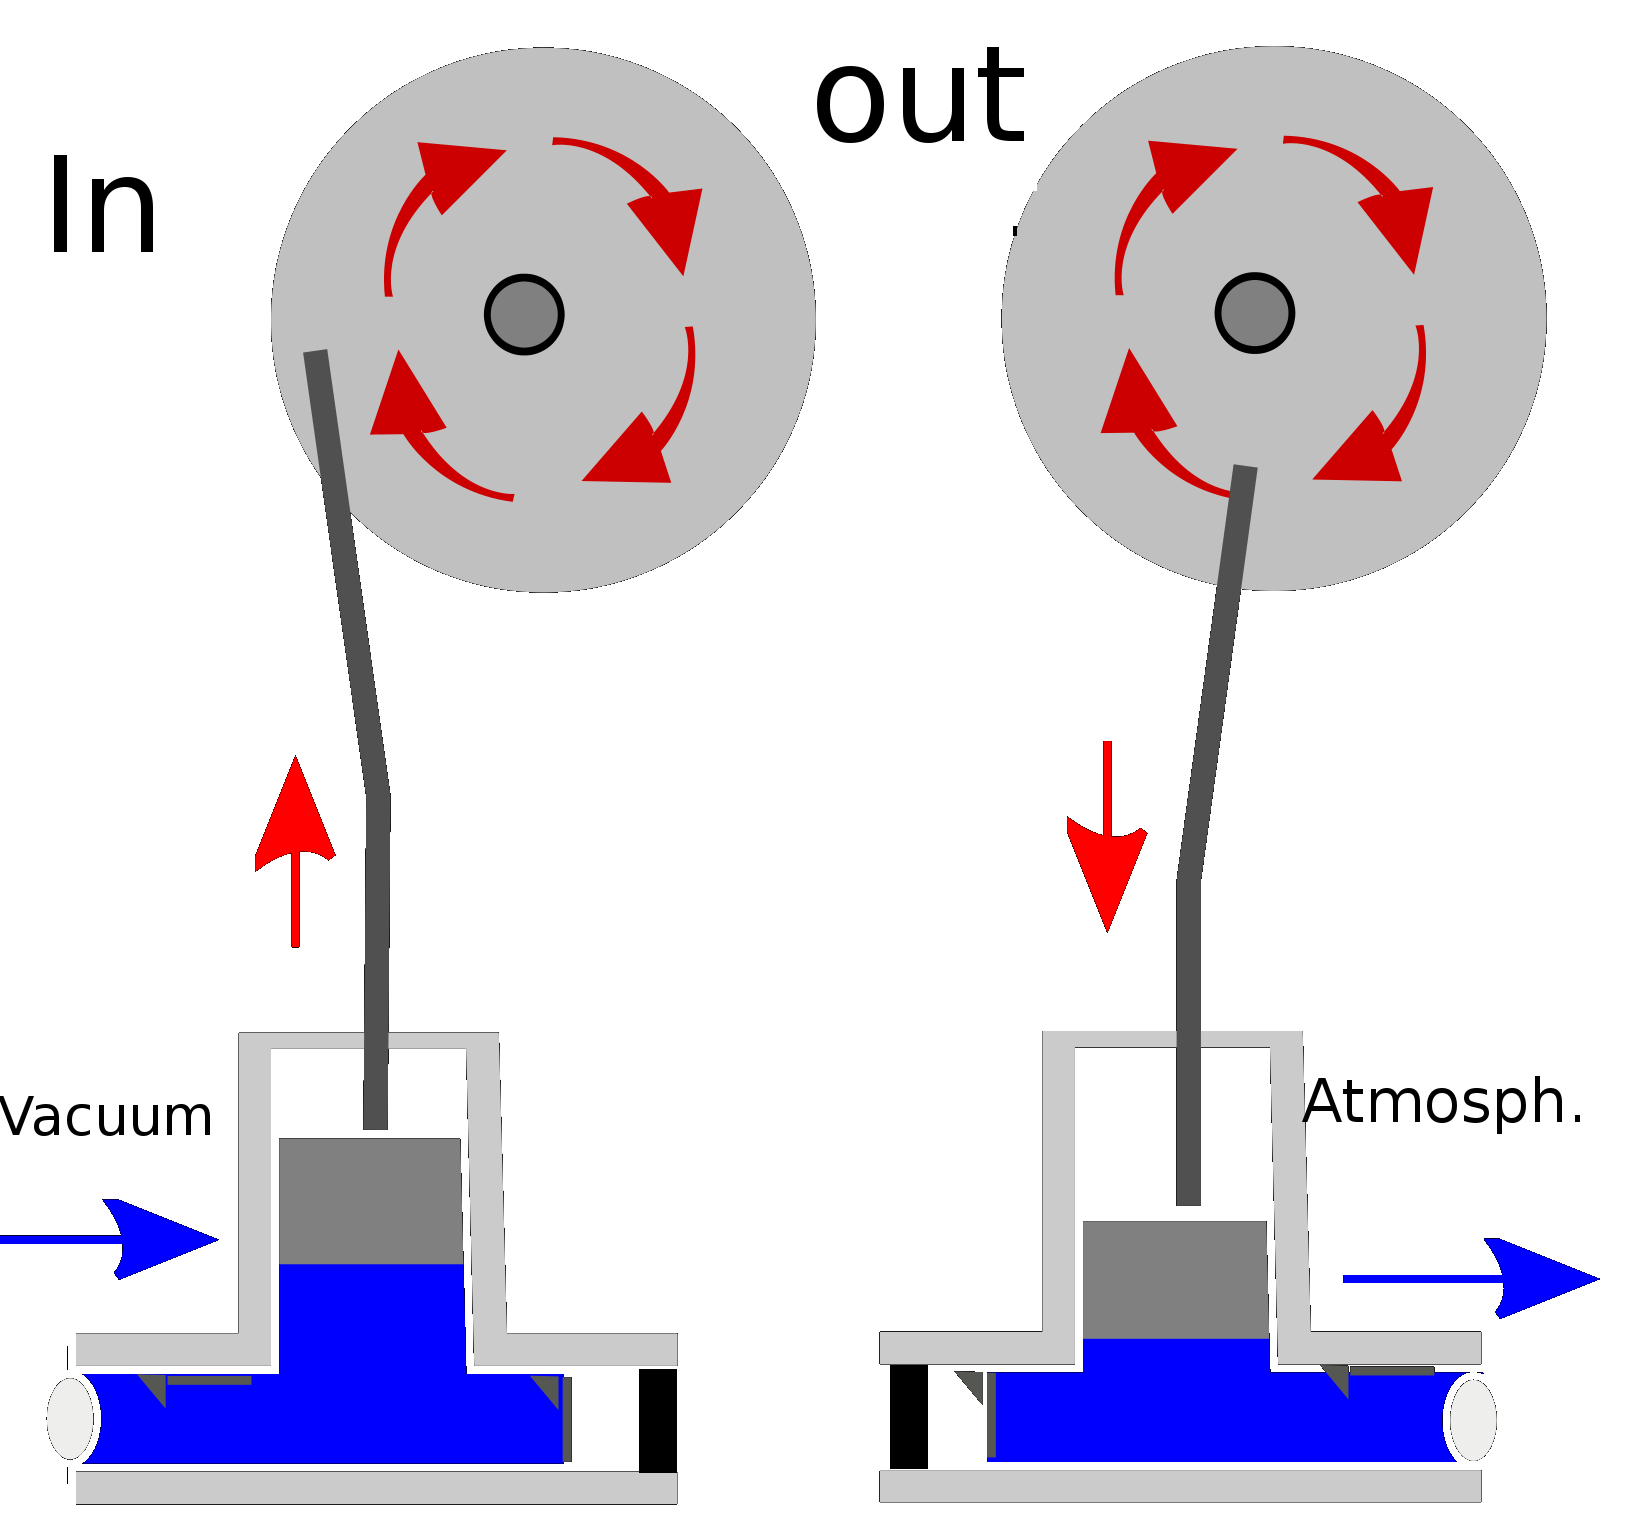
\includegraphics[width=0.7\linewidth]{Bilder/PrePump}
	\label{fig:prepump}
	\caption{Shematic representation of a pump}
	
\end{figure}


The pressure limit we can reach with the pre pump alone is on the one hand caused by leaks of the valves and the piston. On the other hand there is a pressure limit even with perfect valves by the air ($V_{0} $) at atmospheric pressure which remains in the cylinder at the outlet stage . With isotherm expansion in the cylinder we can calculate this minimum pressure to be: \[ p_{min}=p_{Atmosph.}\frac{V_{0}}{V_{max}} \]
\subsubsection{Turbo Pump}
Different from the pre pump which works by producing a pressure gradient between two chambers, a turbo pump works through the principle of momentum transfer. Atoms in a chamber don't bounce elastically of the walls but stick to them through adsorption for a short amount of time, so it is possible to accelerate them with spinning rotors in the turbo pump and push the atoms to the outlet. This only works if the mean free path of a particle is lager than the distance between the rotor blades, which is why we connect the outlet of the turbo, to the pre pump. Our turbo pump is able to evacuate 300 litres of gas per minute.
\subsection{Sputtering}

\subsection{Flow}
\subsubsection{Laminar}
\subsubsection{Turbulent}
\subsubsection{Resistance and Conductivity}
\subsection{Gauges}
\subsection{Questions}
\subsubsection{Day1}
\begin{itemize}  
	\item What causes the limit on the pressure one can reach with the pre-pump alone? $\surd$
	\item  Calculate the mean free path of a nitrogen (N2) molecule in atmospheric pressure and at $1 \cdot 10^{−9}$ mbar 
	\item Based on the data from section 5.3, how much gas is desorped from the walls after the turbo reaches full speed? Hint: Consider the data over the time period after the turbo reaches speed. This is the pressure drop in a fixed time. The volume of the chamber is 30 litres and you can assume the chamber is at a constant temperature of 293K. The mass of air is approximately 29g/mol.
	 

	\item What is the purpose of baking out a chamber? 
	\item What is the thermal energy at room temperature and the corresponding thermal speed of a water molecule (H2O)?
\end{itemize}
\subsubsection{Day2}
\begin{itemize}
	 \item Can you name some properties which might arise due to scaling down the thickness of a sample? \item How have the elemental peaks changed from the spectra of the first day? What can you say about the baking process? How will the baking process affect the quality of the samples being grown? \item Why does the pressure oscillate with clear periods of increasing and decreasing pressures during baking? \item What happens to the plasma as you increase the power being applied to the cathode?
	Page 14 of 34
	\item Why do we pre-sputter the target before deposition? \item  Plot the Polanyi-Wigner equation as a function of desorption energy for an ensemble of $5.35 \cdot 10^{13}$ particles for $T_w$ = 300K, 500K, 800K, 1000K for Edes between 0 and 60 kJ/mol (universal gas constant 8.31 J/mol). Scale the y-axis to $10^{13}$ as a maximum.
	
\end{itemize}
\section{Experiment}
In the experiment we were allowed to operate a vacuum chamber with a volume of 30 litres. The inside is reachable by the main window which is hold by eight bolts and a copper seal. The sputtering targets are at the bottom while a rotatable disk, where the sample was placed, is in the center. This one is operate-able from the outside. At the backside the pressure gauges are connected. 
The chamber itself was connected to a turbo pump, which itself was connected to a valve with electric controls as well a brass cap for the venting. Behind the turbo pump the pre-pump with a 25mm diameter tubing was placed. Above the pumping systems is the mass spectrometer with its filament.

\subsection{Description}
\subsection{Data Analysis}
\subsection{Evaluation}

\end{document}

